\chapter{\label{chap:intro}Introdução}

\sigla{EGCS}{Elevator Group Control System}

Em 2014, 54\% da população mundial vivia em áreas urbanas, de acordo com a Organização das Nações Unidas~\cite{UN14}. A expectativa é que esta proporção aumente para 66\% até o ano 2050. Em números absolutos isto representa um acréscimo de 2,5 bilhões de pessoas à população urbana mundial nos próximos 35 anos. Uma das consequências da alta densidade populacional em regiões geográficas limitadas é o crescimento do modelo de verticalização na construção civil. Neste cenário, onde prédios de diversos andares se tornam presença no cotidiano da maioria da população, os elevadores\footnote{Dispositivos de transporte vertical que movimenta pessoas ou cargas entre andares ou níveis de um prédio ou estrutura.} passam a um papel de destaque.

Uma pesquisa realizada pela IBM no ano de 2010 em 16 cidades norte-americanas constatou que, durante 12 meses, o tempo estimado no qual trabalhadores de escritórios\footnote{Em uma força de trabalho total de 51 milhões de trabalhadores, dos quais 12,7 milhões são usuários de elevadores diariamente~\cite{IBM10}.} aguardaram por elevadores foi de 92 anos~\cite{IBM10}. Em uma economia onde o salário horário médio de um trabalhador é de US\$ 24,99, o tempo de espera por elevadores representa custos de mais de US\$ 20 bilhões em média por ano~\cite{BLS15}.

Além do impacto econômico existe o impacto psicológico. Trabalhadores em centros metropolitanos empreendem uma parcela significativa da sua rotina no deslocamento entre residência e local de trabalho e no caminho inverso ao final do dia. Além de gastar uma quantidade significativa de tempo no trânsito das ruas, em carros, ônibus, bicicletas e metrôs, o tempo compreendido entre aguardar o elevador e desembarcar no andar desejado está longe de ser desprezível. De acordo com reportagem da revista Time, o \textit{everyday commute}, ou \textit{translado casa-trabalho e trabalho-casa} em uma tradução livre, pode causar uma série de efeitos físicos, como aumento nos níveis de açúcar, colesterol e dores nas costas, e psicológicos, como aumento na ansiedade e depressão \cite{Kylstra14}.

\begin{figure}[htb!]
\centering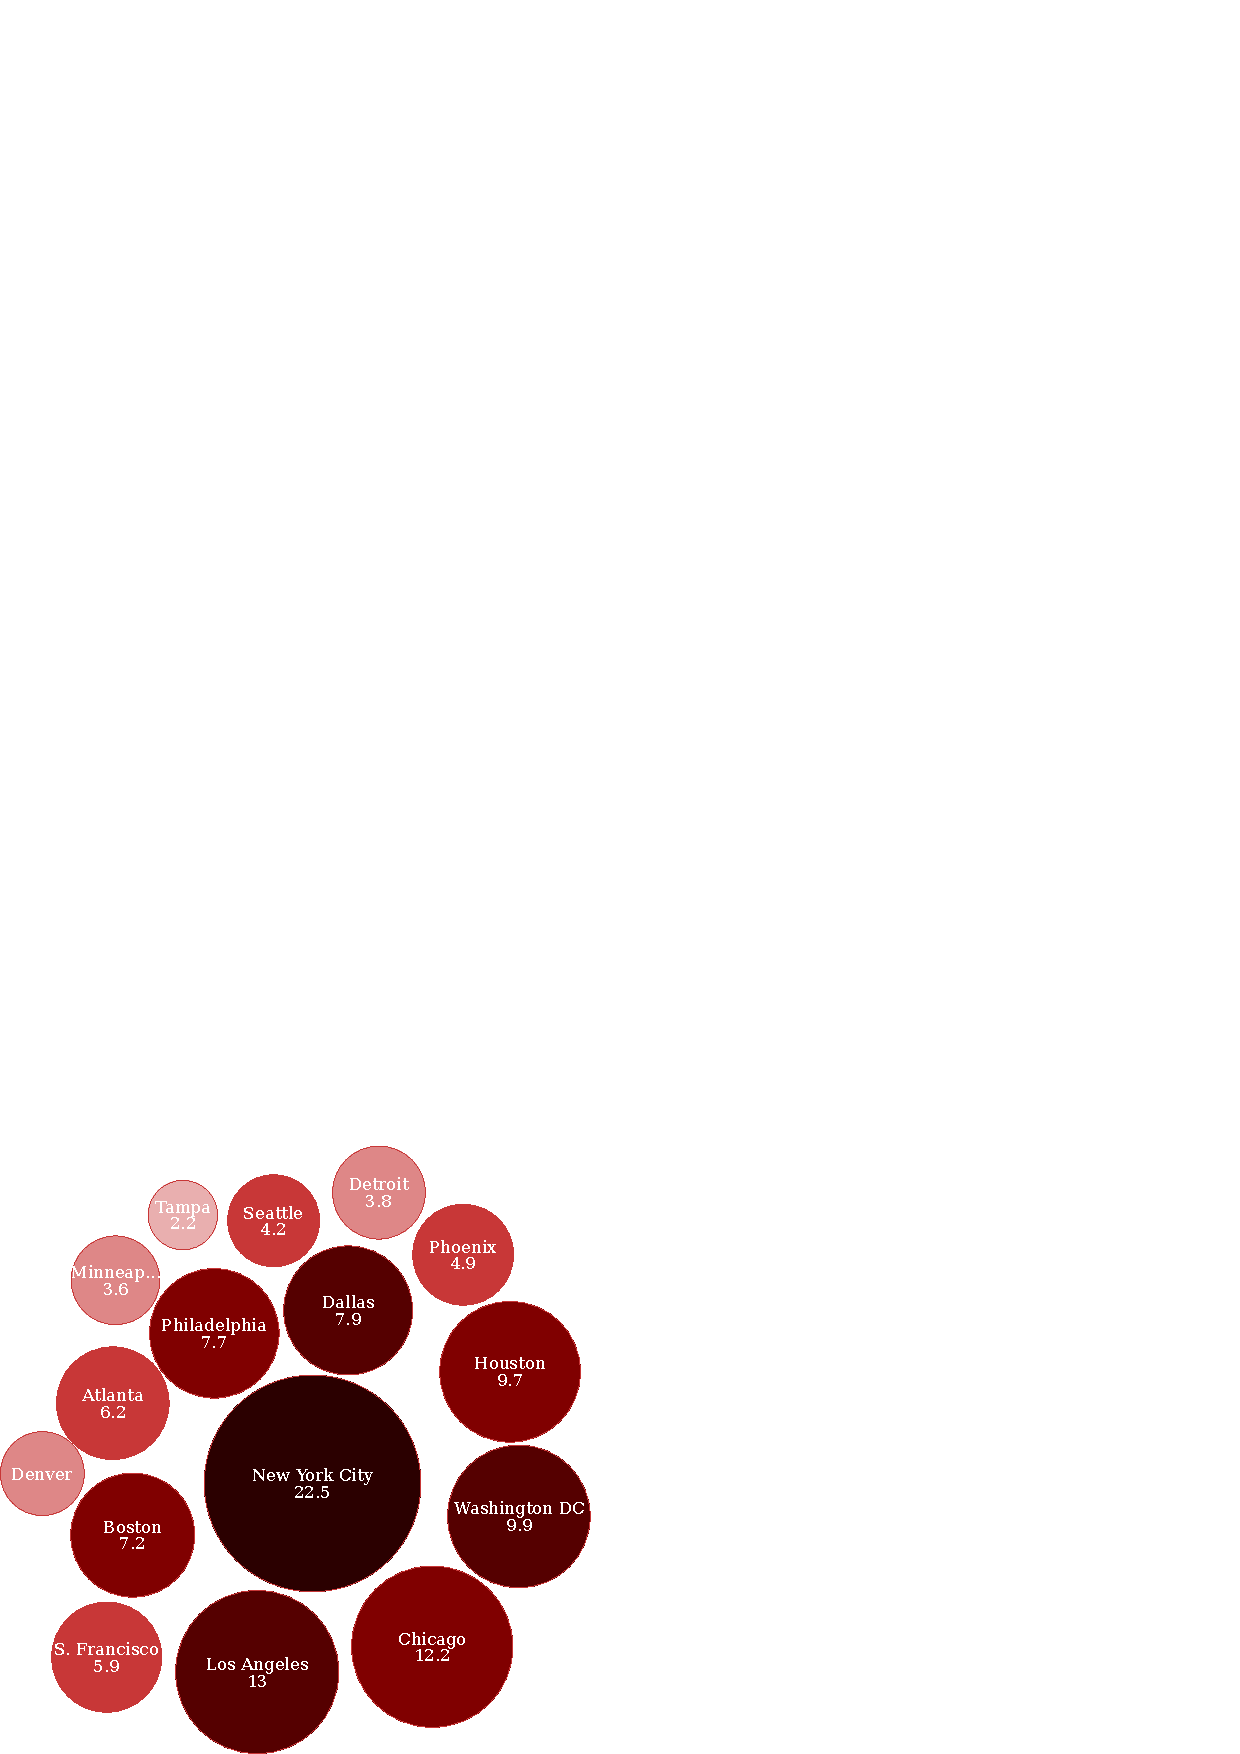
\includegraphics{img/time-cost.jpg}
\caption{\label{fig:fig1}Tempo de espera acumulado (em anos) por elevadores durante 12 meses em 16 cidades norte-americanas. Fonte:~\cite{IBM10}}
\end{figure}

Neste contexto global, a indústria de elevadores possui alguns desafios: primeiro, lidar com a pressão para a redução de custos na construção civil, construindo sistemas de grupos de elevadores mais baratos e eficientes, com melhorias no desempenho de transporte; segundo, competir no mercado oferecendo serviços novos, personalizados e com garantia de qualidade, visando revolucionar a maneira com que elevadores interagem e servem passageiros~\cite{KOEHLEROTTIGER02}. Já sob o ponto de vista dos passageiros, estes esperam que suas chamadas sejam atendidas imediatamente e que sejam levados ao seu destino o mais rápido possível. Portanto, melhorias no desempenho destes sistemas traduzem-se em alto valor tanto para os fabricantes quanto para os usuários de elevadores.

Existem diversas abordagens que os fabricantes de elevadores podem usar para tornar o sistema mais eficiente. Por exemplo, projetar o sistema com um número maior de elevadores ou optar por elevadores com maior capacidade de carga. Entretanto, este tipo de alteração não é sempre realizável em função de limitações na estrutura do prédio ou inviabilidade financeira. Uma solução de mais fácil aplicação é otimizar o sistema de controle dos elevadores.

\section{Sistema de Controle de Grupo de Elevadores}

Um \textit{Elevator Group Control System} (\textbf{EGCS}), ou sistema de controle de grupo de elevadores, é responsável por coordenar as ações de todos os elevadores do prédio~\cite{kuzunuki1984elevator}. Esta coordenação visa atender à todas \textbf{chamadas de corredor}\footnote{Passageiros estão fora dos elevadores e realizam uma chamada para subir ou descer à partir do andar em que se encontram.} e \textbf{chamadas de cabine}\footnote{Passageiros estão dentro do elevador e realizam uma chamada para desembarcar em um andar destino} em cada instante. Para tanto, o EGCS utiliza-se de algoritmos e heurísticas aplicados à dados de entrada que refletem o estado atual do sistema. Estes dados são compostos, minimamente, por:

\begin{itemize}
  \item Para cada andar:
  \begin{itemize}
    \item Se existe uma chamada para subir a partir deste
    \item Se existe uma chamada para descer a partir deste
  \end{itemize}
  \item Para cada elevador:
  \begin{itemize}
    \item O andar em que se encontra
    \item Se está parado, subindo ou descendo
    \item Sua lotação
    \item Um conjunto de paradas solicitadas pelos passageiros
  \end{itemize}
\end{itemize}

A função do EGCS, portanto, trata-se de resolver um problema de otimização: atribuir elevadores para atender chamadas minimizando alguma métrica - veremos mais adiante as métricas de desempenho de um EGCS. Entretanto, este problema encontra-se no conjunto de problemas NP-difícil (ou NP-hard, ou NP-complexo)~\cite{SeKo99}. Portanto, uma solução ótima, decidível em tempo polinomial, ainda não é conhecida para este problema.

Desde meados dos anos 1980, a indústria de elevadores vem estudando e implementando estratégias para encontrar soluções sub-ótimas para o problema. Diversas técnicas de Inteligência Artificial foram adotadas, como redes neurais, algoritmos genéticos, lógicas \textit{fuzzy} e, mais recentemente, sistemas multi-agentes, planejamento e aprendizado de máquina~\cite{KOEHLEROTTIGER02}.


% TODO - vamos fazer o simulador ou usar um pronto? DEFINIR
{\color{red}A proposta deste trabalho é comparar diferentes estratégias de controle de elevadores em alguns cenários e avaliar, dentre as opções possíveis, quais combinações resultam em um melhor desempenho no transporte de passageiros. A comparação se dará analisando os resultados de simulações de diferentes algoritmos de controle. Para tanto, serão implementados no mínimo 2 algoritmos para o sistema de controle de elevadores e um simulador de elevadores. O usuário do simulador poderá:

\begin{itemize}
  \item Selecionar cenários;
  \item Selecionar um algoritmo para controle dos elevadores ou implementar o seu próprio;
  \item Comparar o desempenho entre diferentes algoritmos em um mesmo cenário;
  \item Comparar o desempenho de um algoritmo em múltiplos cenários.
\end{itemize}

Com base nos resultados estatísticos obtidos através das simulações serão realizadas análises quantitativas e qualitativas e, se possível, otimizações nas implementações dos algoritmos. Assim, objetiva-se encontrar quais são as melhores estratégias para cada cenário proposto.}

\section{Motivação Prática}

A Inteligência Artifical é uma área de conhecimento de grande interesse dos autores, junto dos problemas relacionados a simulações, às ferramentas de programação e à engenharia de software. O problema de otimização na alocação de elevadores apresenta um campo de pesquisa único para a aplicação destas ferramentas em busca da prática da Inteligência Artificial.

Além disso, o uso de elevadores é presente na vida de todos os habitantes de grandes metrópoles. Uma parcela significativa do dia-a-dia desta população é passada em grandes caixas metálicas, ou esperando pelas mesmas. A possibilidade de aplicar conhecimentos em Inteligência Artificial para melhorar o desempenho deste meio de transporte e, por conseqüência, contribuir com um aumento na qualidade de vida de seus passageiros é um grande atrativo para a escolha deste tópico.

Ao analisar a tecnologia atual, percebe-se que houve pouca evolução nos elevadores desde sua concepção. De fato, o mecanismo que os faz mover evoluiu drasticamente, quando comparamos elevadores de tração manual com as máquinas modernas. No entanto, tais evoluções são de difícil percepção aos usuários de elevadores. O sistema de controle dos elevadores ainda é simples, utilizando-se muito pouco de técnicas de aprendizado e heurísticas para alterar seu comportamento em tempo de execução. Acredita-se que seja possível trazer uma evolução grande para os sistemas de controle de grupos de elevadores com Inteligência Artificial, assim como os motores elétricos foram para a tração dos elevadores.

Os problemas de simulação também são particularmente interessantes. Definir métricas e realizar a coleta de dados significativos para o problema é um conjunto de habilidades que perdurará e será de inestimável valor profissional e pessoal.